\documentclass[twoside]{article}
\usepackage{amsgen,amsmath,amstext,amsbsy,amsopn,amssymb,color}
\usepackage{graphicx}
\usepackage{epsfig}

\setlength{\oddsidemargin}{0.1 in} \setlength{\evensidemargin}{-0.1
in} \setlength{\topmargin}{-0.6 in} \setlength{\textwidth}{6.5 in}
\setlength{\textheight}{10.5 in} \setlength{\headsep}{0.1 in}
\setlength{\parindent}{0 in} \setlength{\parskip}{0.1 in}

\newcommand{\red}{\textcolor{red}}

\newcommand{\homework}[2]{
   \pagestyle{myheadings}
   \thispagestyle{plain}
   \newpage
   \setcounter{page}{1}
   \noindent
   \begin{center}
   \framebox{
      \vbox{\vspace{2mm}
       \hbox to 6.28in { {\bf Math 4720:~Statistical Methods \hfill} }
       \vspace{6mm}
       \hbox to 6.28in { {\Large \hfill #1 (#2)  \hfill} }
       \vspace{6mm}
      \vspace{2mm}}
   }
   \end{center}
   \markboth{#1}{#1}
   \vspace*{4mm}
}

\newcommand{\bbF}{\mathbb{F}}
\newcommand{\bbX}{\mathbb{X}}
\newcommand{\bI}{\mathbf{I}}
\newcommand{\bX}{\mathbf{X}}
\newcommand{\bY}{\mathbf{Y}}
\newcommand{\bepsilon}{\boldsymbol{\epsilon}}
\newcommand{\balpha}{\boldsymbol{\alpha}}
\newcommand{\bbeta}{\boldsymbol{\beta}}
\newcommand{\0}{\mathbf{0}}

\begin{document}

\homework{$13^{th}$ and $14^{th}$ Week Summary}{04/25/25}
\vspace{-0.4 in}
\begin{itemize}
\item \textbf{Chi-square Tests}\dotfill
\item The \textbf{chi-square goodness-of-fit} test allows us to test whether a categorical variable follows a given probability distribution.
\item A categorical variable has $k$ possible outcomes, with probabilities $\pi_1, \pi_2, \pi_3, \ldots, \pi_k$. That is, $\pi_i$ is the probability of the $i^{th}$ outcome. We have $n$ independent observations from this categorical variable.
\item We use chi-square goodness-of-fit test for testing the null hypothesis that the probabilities have specified values:
\subitem $H_0: \pi_1={\pi_1}_0, \pi_2={\pi_2}_0, \pi_3={\pi_3}_0, \ldots, \pi_k={\pi_k}_0$
\subitem The expected count of outcome $i$, $E_i=n{\pi_i}_0$. Expected counts do not have to be round numbers.
\item The chi-square statistic is a measure of how far observed counts are from expected counts under the null hypothesis. The formula for the statistic is:
\subitem $\chi^2=\sum{\dfrac{(\textrm{observed count - expected count})^2}{\textrm{expected count}}}=\sum_{i=1}^k{\dfrac{(O_i-E_i)^2}{E_i}}$
\subitem Each of the k terms in the sum is called a chi-square component
\item The chi-square goodness of fit test involving $k$ outcomes refers to the chi-square distribution with $k - 1$ degrees of freedom. The p-value is the area to the right of $\chi^2$ under the density curve of this chi-square distribution.
\item You can safely use the chi-square goodness-of-fit test with critical values from the chi-square distribution when no more than $20\%$ of the expected counts are less than $5$ and all individual expected counts are $1$ or greater. In particular, the chi-square goodness-of-fit test can be used when all the expected counts are $5$ or greater.
\item The \textbf{chi-square test of independence} is for checking the dependence of two categorical variable. The null hypothesis is given by :
\subitem $H_0:$ Two categorical variables are independent of each other.
\item The chi-square test for a two-way table with $r$ rows and $c$ columns uses critical values from the chi-square distribution with $(r - 1)(c - 1)$ degrees of freedom.
\item You can safely use the chi-square test with critical values from the chi-square distribution when no more than $20\%$ of the expected counts are less than $5$ and all individual expected counts are $1$ or greater. In the special case of a $2 \times 2$ table, all four expected counts should be $5$ or greater.
\item \textbf{Regression}\dotfill
\subitem A tool to describe how a response (dependent) variable \(y\) changes based on an explanatory (independent) variable \(x\). Often, a straight line is used to model and predict \(y\) given \(x\).
$$y_i = \beta_0 + \beta_1 x_i + \epsilon_i,$$
where \(\epsilon_i\) are normally distributed error terms with mean 0 and constant variance \(\sigma^2\).
\item Least Squares Estimation: 
\subitem The slope \(\hat{\beta}_1\) and intercept \(\hat{\beta}_0\) are chosen to minimize the sum of squared residuals, \(\sum (y_i - \hat{y}_i)^2\).
\item Assumptions:
\subitem Linear relationship between \(x\) and \(y\).
\subitem Independent, normally distributed error terms with constant variance.
\subitem Watch for outliers or influential points that may distort the regression.

\newpage

\item ANOVA and \(\boldsymbol{R^2}\):
\subitem An ANOVA table splits total variation into that explained by the regression and that attributed to error. The coefficient of determination \(R^2\) measures the proportion of the variation in \(y\) explained by the model.

\item Inference:
\subitem Hypothesis tests (e.g., \(H_0: \beta_1 = 0\)) determine whether there is a statistically significant linear relationship. Confidence and prediction intervals provide estimates for the mean response and for individual new observations.
\item Cautions:
\subitem Regression lines only capture linear patterns; always check scatterplots.
\subitem Extrapolating far beyond observed \(x\)-values can be unreliable.
\subitem Residual plots are crucial for checking model assumptions.
\begin{figure}[h]
\begin{center}
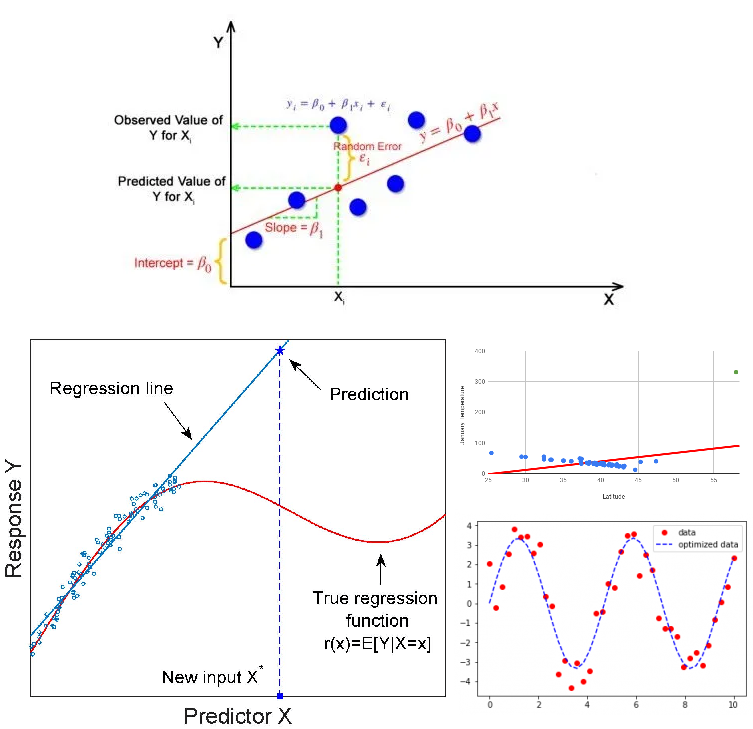
\includegraphics[angle=0, width=\textwidth] {regression.png}
\end{center}
\end{figure}
\end{itemize}
\end{document}
